\chapter{Cloud- Radio Access Networks}
\section{Motivation from LTE to NR5G} Modern applications require the cellular network to be expanded into different services for example IoT Internet of things, mission-critical services, and
V2X services. Development of 4G core network i.e. evolved packet core was
pretty much smartphones-centric. If we use EPC for both smartphone apps
and the IoT apps there will be too much load on the network. To get-off this
load, re-evolution of the EPC to handle different services like V2X, IoT, and
mission-critical services.
Deriving forces behind the next-generation system architecture are. The
introduction of these three factors will enable the following things.

\begin{figure}[h!]
\centering
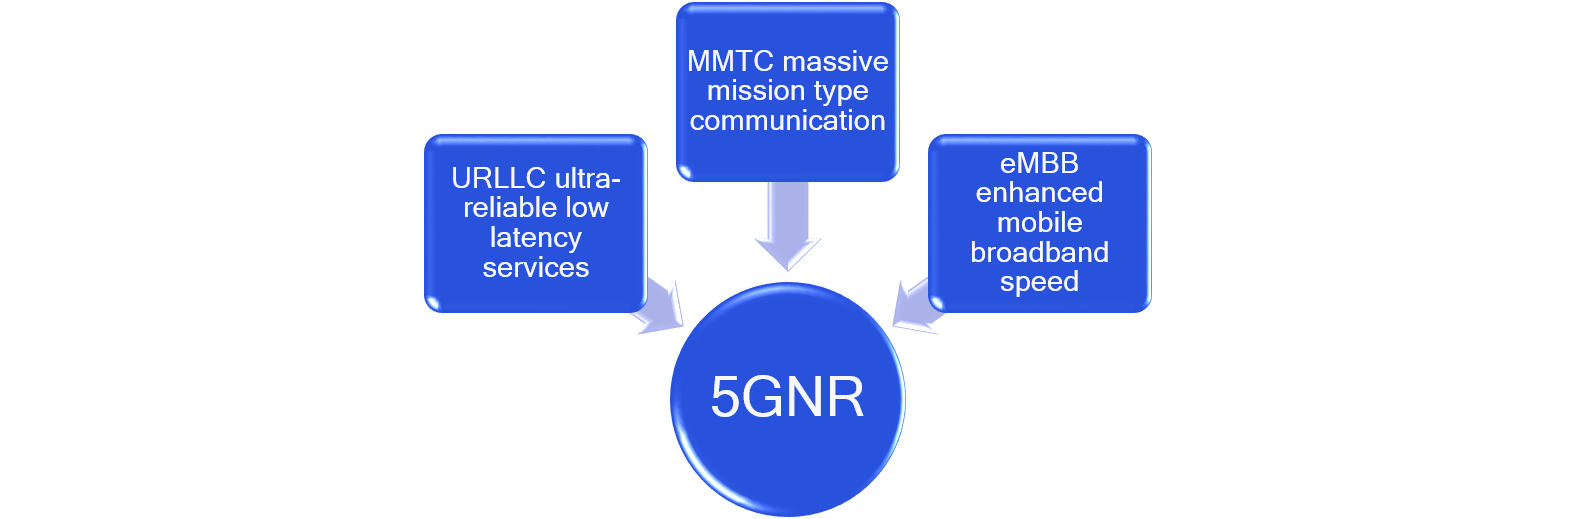
\includegraphics[width=1.0\textwidth]{pic-one.png}
\caption{Promised services by NR5G }
\end{figure}

\begin{enumerate}
    \item Diversified service requirement for URLLC ultra-reliable low latency
services, MMTC massive mission type communication, and eMBB enhanced mobile broadband speed i.e till 20 Gbps.
    
    \item To allow independent and flexible software-hardware evolution. In EPC
hardware and software are fixed. 5G core network is designed in such
a way to easily scale a network by buying some servers and writing
software on the top of it
    
    \item To deploy network functionalities on demand for example to meet the
capacity requirement during a concert by adding a few more nodes.
    
    \item To support more advanced information technology and internet technology
     \item To provide new services rapidly, including design, deployment, and OM.
    \end{enumerate}

\section{Cloud RANs: Service based architecture enablers} 
As discussed in the previous section that the main motivation of having a fifth-generation network is to have a service based scalable architecture. NR5G promises three major application based services. With applications requiring huge amounts of data rates like augmented reality and virtual reality application the services to be fulfilled is eMBB. Massive mission types communication also known as MMTC services requires moderate data rates but more reliability in terms of connectivity and packet delivery. The third type of service is very critical in terms of latency. For example small ultra low power consuming sensors inside the soil of the field constantly transmit data to the fusion system collectively in a swarm over a large area. These sensors barely require any data rate but there is a crucial need to successfully transmit the sensor data with a very low latency over a long period of time. This kind of application based service has been the main deliverable of NR5G in the release 16 and 17. To configure the network with such a flexibility, the cloud based radio access networks or C-RANs have been designed. A typical representation of a C-RAN is shown below in figure 2.

\begin{figure}[h!]
\centering
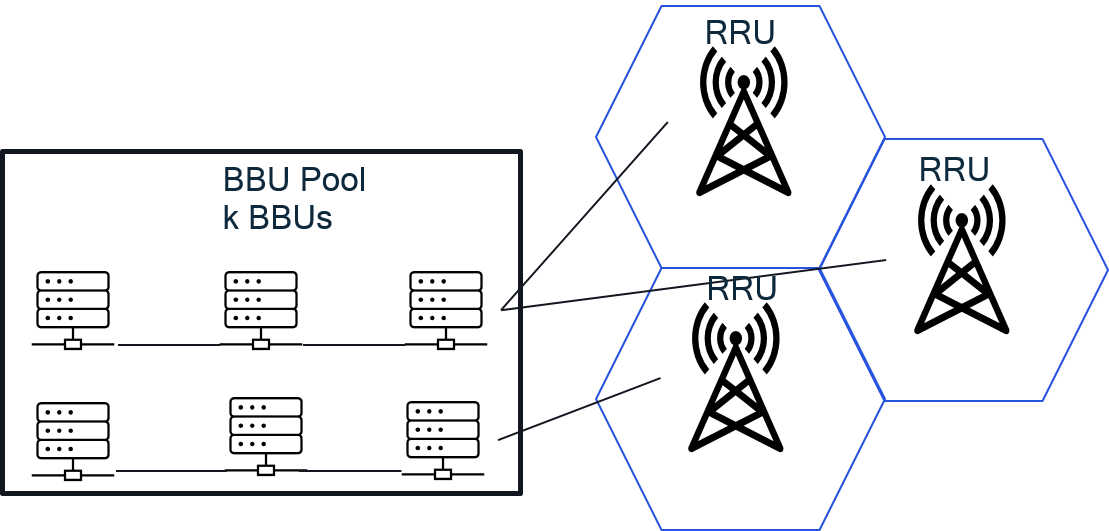
\includegraphics[width=1.0\textwidth]{pic-2.png}
\caption{Typical architecture of a cloud based Radio access network }
\end{figure}

Due to more penetration of the more advances user equipment, the current wireless network is under strain to keep up with the decided key performance indices or KPIs. To mitigate this gap between demand and the delivery, the network operators are propagating towards more denser and smaller cellular structures like femto-cells and pico-cells in case of mmWaves. But these RANs or radio access networks must be able to fulfill not only the demands of advanced network but also must support the legacy networks like LTE, GSM, WCDMA and LTE-A. To enable this kind of inter-operaility with the minimum delay along the overhead calculation and to perform the key operations like scheduling, beamforming, dynamic spectrum sharing, coordinated scheduling, hybrid backhauling, engineers came up with a centralized computing unit which is simply a cloud. On hardware, the solution is to virtualize the processors in the shared resource to perform parallel processing to efficiently mitigate the stress due to various heterogeneous application based services and legacy network services. These virtul machines on a shared hardware resource is are known as baseband unit or BBU and collectively known as the BBU pool as shown in figure 2 above.  This cloud is rather a cluster of servers installed not too far away from the radio resource units RRUs either wirelessly or with wires. To mitigate the delay in scheduling this cloud also known as central unit has enabled virtual machines which efficiently performs the scheduling, encoding, decoding, and resource allocation tasks on the network side. \\
It has been observed that the most of the power consumption on the network side is basically consumed into the baseband processing means once the signal is demodulated corrected by the physical layer, most of the power consumption is done in the baseband domain for the various signal processing steps, encoding and decoding of the transmitted and received signals respectively. From the network operator point of view, power consumption on the network side is directly proportional to the cost. So the most important step towards cost saving from the network side is the reduction in the power consumption.

\section{Challenges in the implementation of C-RAN} Cloud based RAN is a novel idea and already has been implemented. But the main challenge is to perform this optimization in terms of power, latency based on the demanded service from the UE side or IoT devices  